\section{Introduction}

R-Pulsar is build uinsg Java and the open source project TomP2P. TomP2P is a P2P library and a distributed hash table (DHT) implementation which provides a decentralized key-value infrastructure for distributed applications. Each peer has a table that can be configured either to be disk-based or memory-based to store its values.

%TomP2P stores key-value pairs in a distributed manner. To find the peers to store the data in the distributed hash table, TomP2P uses an iterative routing to find the closest peers. Since TomP2P uses non-blocking communication, a future object is required to keep track of future results. This key concept is used for all the communication (iterative routing and DHT operations, such as storing a value on multiple peers) in TomP2P and it is also exposed in the API. Thus, an operation such as get or put will return immediately and the user can either block the operation to wait for the completion or add a listener that gets notified when the operation completes.

The overall operation of the overlay consists of two phases: bootstrap and running. During the bootstrap phase (or join phase), messages are exchanged between a joining RP and the rest of the group. During this phase, the joining RP attempts to discover RPs already existing in the system to build its routing table. The joining RP sends a discovery message to the group. If the message is unanswered after a set duration (in the order of seconds), the RP assumes that it is the first in the system. If an RP responds to the message, the joining RP and the rest of the RPs update their routing tables.

The running phase consists of stabilization and user modes. In the stabilization mode, an RP responds to queries issued by other RPs in the system. The purpose of the stabilization mode is to ensure that routing tables are up to date and to verify that other RPs in the system have not failed or left the system. In the user mode, each RP interacts at the ARMS layer. The ARMS matching engine at each RP is based on ....

Once the system is operating in user mode, RPs allow external entities to use the ARMS layer to communicate with each other to offer and request data and computation. These entities can include: a) users that might want to retrieve specific data or perform certain computation over data found using a query; b) IoT devices that can produce and consume data based on specific interests; and c) computational resources, such as data analytics and streaming platforms, clouds, or high performance computing clusters that offer their computational capabilities.



R-Pulsar as indirect replication which is inherited from TomP2P. The indirect replication can be described as peers publishing content for others. The peer closest to a location ID is considered as the responsible peer and replicates data if necessary. Indirect replication is triggered by two events:

One event is if a peer x gets to know a new peer y. Then peer x checks all its stored data for which peer x is responsible for. If peer y is the new responsible for this stored data, the content will be handed over to peer y and peer y will be the new responsible peer. If peer y leaves the system that was responsible for content and peer x becomes the new responsible peer.

The second event is triggered by a timer. Peer x checks periodically all stored data for enough replicas in the network. If not enough replicas are stored on peers, peer x starts to replicate the content.

\section{API Examples}

The first example uses the resource actions for enabling the exchange of data, without prior knowledge between devices. In Listing~\ref{lst:sensor}, an advertising profile is specified by the drone sensor with the type of data it can produce, and requests to be notified when someone is interested in such data.

\begin{lstlisting}[language=mylang, caption={Data producer resource profile sample code.}, captionpos=b, label={lst:sensor}]
1 profile.addSingle("Drone").addSingle("LiDAR");
2 ARMessage msg = ARMessage.newBuilder()
  .setAction(ARMessage.NOTIFY_INTEREST)
  .setLatitude(40.0583).setLongitude(-74.4056))
  .setProfile(profile);
3 producer.post(msg);
\end{lstlisting}

Respectively, a data consumer declares the type of content of its interest. Listing~\ref{lst:ed} presents a data consumer with interest for any LiDAR sensor data that match the profile ``Drone" and ``Li*", located within the specified range (40*, 70*). As this profile matches the previous profile, the sensor from Listing 1 is notified that there is a consumer interested in its data, then the sensor starts streaming.

\begin{lstlisting}[language=mylang, caption={Data consumer resource profile sample code.}, captionpos=b, label={lst:ed}]
1 profile.addSingle("Drone").addSingle("Li*")
  .addSingle("lat:40*").addSingle("long:-74*");
2 ARMessage msg = ARMessage.newBuilder()
  .setProfile(profile).setAction
  (ARMessage.NOTIFY_DATA);
3 producer.post(msg);
\end{lstlisting}

As mentioned previously, profiles can be used in two different ways: for discovering resources or subscribing to data publishers (resource actions) and for deploying data-processing tasks across the edge and the cloud (function actions). Listing~\ref{lst:ed2} implements the deployment of a function (post\_processing\_func) in the system. This allows the developer to specify where/on which set of resources it should be deployed.

\begin{lstlisting}[language=mylang, caption={Store post-processing task in the R-Pulsar overlay network.}, captionpos=b, label={lst:ed2}]
1 profile.addSingle("post_processing_func");
2 ARMessage msg = ARMessage.newBuilder()
  .setProfile(profile).setLocationTag("Cloud");
  .setAction(ARMessage.STORE_FUNCTION);
3 producer.post(msg);
\end{lstlisting}

Consequently, a profile and a decision (the IF-THEN rule) can be created to decide \textbf{when} to trigger the data-processing function (post\_processing\_func). In Listing~\ref{lst:t-rule}, the resulting action is created and attached to the function profile from Listing~\ref{lst:t-start2}, which is sent when the rule is satisfied.

In addition, Listing~\ref{lst:t-rule} defines a rule that is constantly evaluated for every data element. If the condition of this rule is met, then the function profile from Listing~\ref{lst:t-start2} is forwarded, resulting in the execution (trigger) of the data-processing task previously stored.

\begin{lstlisting}[language=mylang, caption={Rule based programming abstraction for deploying the post-processing task.}, captionpos=b, label={lst:t-rule}]
1 Action topo1 = new Reaction(T-profile);
2 Rule rule1 = new Rule.Builder()
  .withCondition("IF(RESULT >= 10)")
  .withConsequence(topo1).withPriority(0);
\end{lstlisting}

\begin{lstlisting}[language=mylang, caption={Profile for deploying the post-processing task.}, captionpos=b, label={lst:t-start2}]
1 T-profile.addSingle("post_processing_func");
2 ARMessage msg = ARMessage.newBuilder()
  .setAction(ARMessage.START_FUNCTION)
  .setProfile(T-profile);
3 producer.post(msg);
\end{lstlisting}

\section{Location-aware Overlay Network Layer Evaluation}

%\section{Evaluation}
%In this section all the layers of R-Pulsar are evaluated by using three metrics: Overhead, Scalability and Performance. In addition each of those experiments are evaluated using cloud resources and Edge devices:

%\begin{itemize}
%\item Edge System: Using Raspberry Pi 3 with 4x ARM Cortex-A53 1.2GHz, 1GB LPDDR2 of RAM and 10/100 Ethernet.
%\item Cloud System: Chameleon Cloud~\cite{chameleon}, a configurable experimental environment for large-scale cloud research~\cite{chameleon}, with 5 instances of type m1.small (1 CPU and 2 GB RAM) and 5 instances of type m1.medium (2 CPU and 4 GB RAM) to simulate the computation capabilities of a Raspberry Pi and the hardware heterogeneity that IoT presents.
%\end{itemize}

In this section we evaluate the overhead and scalability of the location-aware overlay network layer of R-Pulsar. The tests are evaluated using cloud resources and Edge devices:

\begin{itemize}
\item Edge System: Using Raspberry Pi 3 with 4x ARM Cortex-A53 1.2GHz, 1GB LPDDR2 of RAM and 10/100 Ethernet.
\item Cloud System: Chameleon Cloud~\cite{chameleon}, a configurable experimental environment for large-scale cloud research~\cite{chameleon}, with one RP deployed in a type m1.medium (2 CPU and 4 GB RAM) instance.
\end{itemize}

\subsection{Overhead and Scalability Over Cloud And Edge Systems}

This experiment measures the overhead involved in performing a location-based query to identify relevant resources around the location of a client node. In our experiments, the location-based query used the GPS coordinates of each RP node and the client to identify the RP around the client.
%As we described in Figure~\ref{fig:example1A}, a location-based query involves sending {\it statistics} action messages to all RP with a matching location, which ask RPs to send their information to the client. In these experiments, we only measured the overhead incurred in querying the database and constructing the ``notify\_interest'' message, i.e., the notification delivery was not measured. For these experiments, we had a total of 1000 RP nodes and we varied the position of the client, resulting in a different number of RP nodes matching the location requirement. Figure~\ref{fig:matching} collects the results of these experiments.

\begin{figure}[htb!]
  \centering
    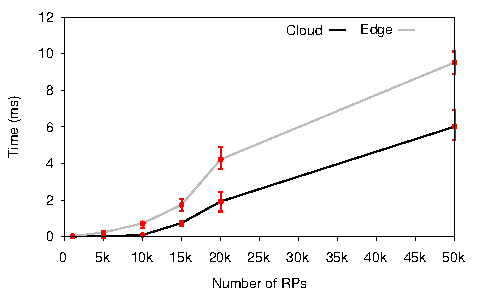
\includegraphics[width=0.8\textwidth]{Figures/OSLocation.pdf}
  \caption{Location-based query overhead for different number of matches per query.} \label{fig:oslocation}
\end{figure}

Figure~\ref{fig:oslocation} shows that the overhead of performing a location-based query increases ... as the number of RP nodes in the system increases. Results show a maximum overhead of 10 milliseconds, which occurred when 50k RPs are in the system. 

\subsection{Overhead and Scalability of the Data Replication}

Next, we measured the time required to replicate the information stored across a set of RP nodes in the system. In these experiments, we considered several scenarios involving different number of RP nodes as well as different number of replication factors. Figure~\ref{fig:topology} collects the results. 

\begin{figure}[htb!]
  \centering
    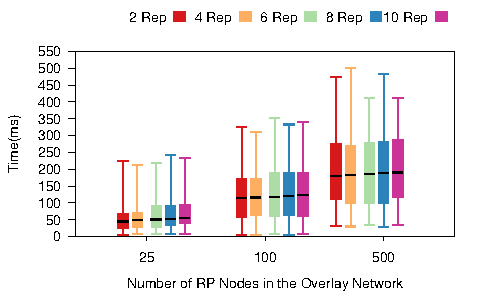
\includegraphics[width=0.8\textwidth]{Results/ReplicationOver.pdf}
  \caption{Time neccessary to update information of all RP nodes in the system after multiple topologies are registered.} \label{fig:topology}
    \vspace{-2ex}
\end{figure}

We can observe that in Figure~\ref{fig:topology} that the time required to replicate the information across all the RP nodes in the system is relatively low. In particular, it can vary from a few milliseconds to around 200 milliseconds on average when having a large system with 500 RP nodes. The main factor affecting the time required to propagate the information is the number of RP nodes, since the time to route a message increases. 

\section{Content-based Routing Layer Evaluation}

In the content-based routing layer we evaluate three aspects: The first aspect is the overhead of matching profiles, The second aspect we evaluate is the overhead and scalability of the routing, and finally we evaluate the propagation of ....  The tests are evaluated using the same cloud and edge resources as described in the previous section.

\subsection{Profile Matching Overhead Over Cloud Systems}

This first experiment measures the overhead involved in the profile matching operation at an RP node. We used a {\it notify\_data} action message for these experiments. We considered different scenarios in which the system had different number of data profiles (i.e. subscriptions) and the request returned a different number of profile matches. As we described in Figure~\ref{fig:example1B}, a {\it notify\_data} request asks an RP to find matching profiles and to send a {\it notify} message to the profile owners -- e.g., requesting to start streaming data. In this experiment, we measured the overhead of performing the matching operation and constructing the ``notify'' messages.  The experiment was conducted using profiles similar to the one described in Figure~\ref{fig:profiles}, which contains sets of complex keyword tuples containing wildcards and/or ranges. Figure~\ref{fig:profileQuery} collects the results of these experiments. 

\begin{figure}[htb!]
  \centering
    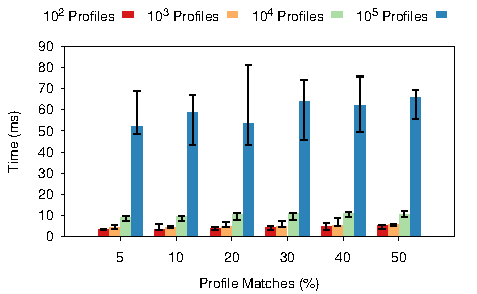
\includegraphics[width=0.8\textwidth]{Figures/profileQuery.pdf}
  \caption{Profile matching overhead. Results are grouped based on the matching ratio expressed as a percentage of the total number of stored profiles.} \label{fig:profileQuery}
\end{figure}

We can observe in Figure~\ref{fig:profileQuery} that, for a moderate database size of up to $10^4$ profiles, the profile-matching operation incurs in an overhead between five and 10 milliseconds. Nonetheless, when we increase to $10^5$ profiles, the overhead increases significantly, as could have been expected given the memory and data access times required to identify and retrieve such a large number of profiles. As a consequence, we need to ensure that the number of profiles that each RP manages is within a manageable range to minimize the overheads. This can be achieved by implementing load-balancing techniques and limiting the knowledge of each RP to its closest neighbors. 


\subsection{Routing Overhead and Scalability Over Edge Systems}

This second set of experiments measure the routing overhead, which represents the time interval between an AR message is created until it is forwarded to the recipient of the message. It is important to maintain the routing overhead in the order of milliseconds to achieve real-time analytics on constrained devices. The routing overhead was evaluated over Android and Raspberry PIs by simulating the storage or retrieval of data, as the number of RPs on a given region grows, and also as the AR profiles complexity grows. The profile complexity is defined in terms of the number of attribute-value pairs that make up the profile. For example, a 2D profile is composed of two properties, such as data type and location.

\begin{figure}[h!]
  \centering
  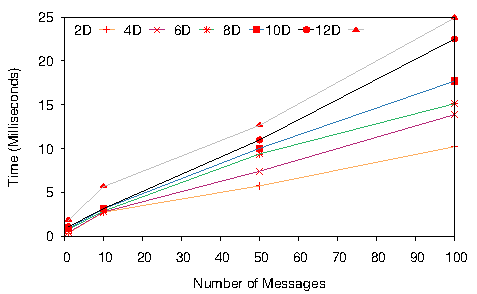
\includegraphics[width=0.8\textwidth]{Results/Phone}
  \caption{Evaluation of R-Pulsar space filling curve routing overhead and scalability as the number of messages and the complexity of profiles increase over the Android system.}
  \label{fig:Phone}
\end{figure}

\begin{figure}[h!]
  \centering
  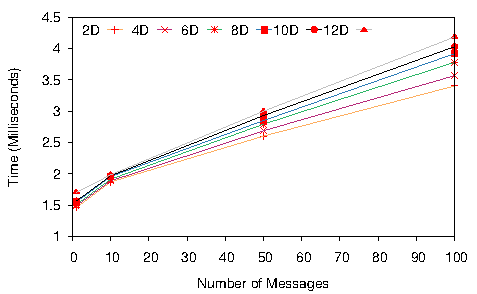
\includegraphics[width=0.8\textwidth]{Results/Raspberry}
  \caption{Evaluation of R-Pulsar space filling curve routing overhead and scalability as the number of messages and the complexity of profiles increase over the Raspberry Pi system.}
  \label{fig:Raspberri}
\end{figure}

Figure~\ref{fig:Phone} shows that when the profile complexity increases by a factor of 6, the time required to route messages increases by 2.5. Similarly, when the system increases the number of messages sent by a factor of 100, the time required to route one message increases by a factor of 25. It shows that the routing overhead scales efficiently in both cases, as messages become increasingly complex and as the number of messages sent increases when using the Android system. 

However, Figure~\ref{fig:Raspberri} shows that when the profile complexity increases by a factor of 6, the time required to route messages increases by about 1.2, when using the Raspberry Pi system. Likewise, when the system increases the number of messages sent by a factor of 100, the time required to route one message increases by about 2.5. Demonstrating that the routing overhead scales more efficiently on a Raspberry Pi system than on an Android system.
\vspace{1ex}

%\subsection{Routing Overhead and Scalability Over Cloud Systems}

%\begin{figure}[h!]
%  \centering
%  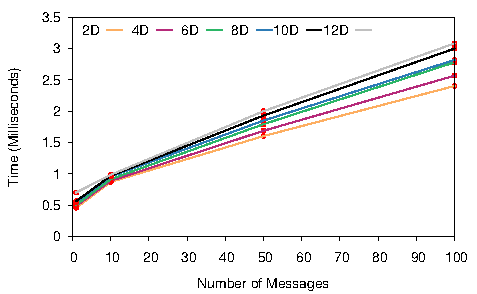
\includegraphics[width=0.8\textwidth]{Results/Cloud.pdf}
%  \caption{Evaluation of R-Pulsar space filling curve routing overhead and scalability as the number of messages and the complexity of profiles increase over a Cloud system.}
%  \label{fig:Raspberri}
%\end{figure}


\subsection{Information Propagating through the System}

This last set of experiments are performed to understand the behavior of the system when multiple RP nodes request to join an existing deployment of our system. Specifically, we measured the time from when the RP nodes sent their joint message until all RP nodes existing in the system were updated. In our experiments, we varied both the number of RP nodes wanting to join and the number of existing RP nodes in the system. Figure~\ref{fig:rpDiscovery} collects the results.

\begin{figure}[htb!]
  \centering
    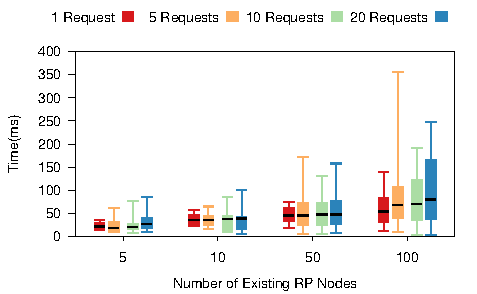
\includegraphics[width=0.8\textwidth]{Figures/rpDiscoveryBox.pdf}
  \caption{Time neccessary to update information of all RP nodes in the system after multiple new RP nodes join.} \label{fig:rpDiscovery}
\end{figure}

Figure~\ref{fig:rpDiscovery} shows that the time required to have a consistent view of all the new RP nodes after the requests are placed is relatively low, and that it scales properly when increasing the number of existing RP nodes. In the case of a small system with only five existing RP nodes the overhead is around 20 milliseconds on average. The overhead increases to around 70 milliseconds in the case of having a large system with 100 existing RP nodes. Additionally, we can observe that varying the number of requests does not significantly affect the time required to propagate the information in a system with up to 50 RP nodes. In the case of having 100 RP nodes, we observe that increasing the number of requests, increases the overhead as well as the dispersion around the average. Although it is important to maintain an updated view of the system to ensure that we can efficiently process clients' requests, it is not critical for the regular operations of the system. Our system has mechanisms to adapt to changes in the availability of RP nodes to improve data processing efficiency. Therefore, we consider that having an eventually consistent system is sufficient. 



\section{Serverless Messaging Layer Evaluation}

\section{Memory-mapped Streaming Analytics Pipeline Evaluation}

In this section we evaluate two of the pieces that memory-mapped streaming analytics pipeline consists, the Data collection and the storage and query layers. The tests are evaluated using the same cloud and edge resources as described in the previous section.

\subsection{Performance of the Data Collection Layer Over Edge Systems}

The first experiment aims to evaluate the throughput of R-Pulsar messaging layer. This experiment was carried out using two Raspberry Pi's one as a producer and the other as the broker. The workload sizes are chosen based on the current limitations imposed by existing IoT services, such as AWS~\cite{AWS-MQTT} and Azure~\cite{AZURE-MQTT}. The inner memory-mapped queue is compared to Apache Kafka and Mosquitto. Apache Kafka (the \textit{de facto} standard for cloud and edge data analytics)~\cite{Young2017, firework, planner}, Mosquitto (a broker that can be found on edge frameworks, such as Azure IoT or the AWS Greengrass), and the R-Pulsar memory-mapped queue, using four different message sizes.  The main difference between them is the way they store information: Apache Kafka and Mosquitto store messages on the disk while R-Pulsar stores them in the main memory and disk. 

\begin{figure}[h]
  \centering
  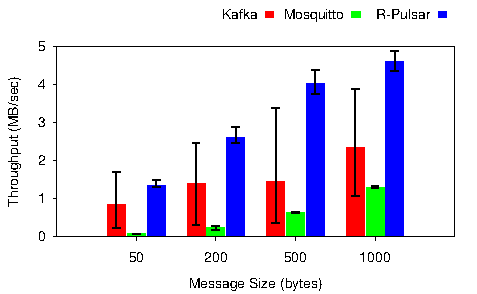
\includegraphics[width=0.8\textwidth]{Results/ProducerBar}
    \caption{Single broker and producer throughput performance as message sizes grow. Comparison of R-Pulsar, Kafka, and Mosquitto systems deployed on a single Raspberry Pi.}
  \label{fig:ProducerBar}
\end{figure}

Results in Figure~\ref{fig:ProducerBar} show that R-Pulsar's throughput scales as the message size increase. This experiment is representative of a traditional IoT scenario with small messages streamed at a high rate arrival.
We observed that R-Pulsar pub/sub messaging system outperforms Kafka by a factor of 3x and Mosquitto by a factor of 7x. Also, Apache Kafka exhibits a high variability of throughput performance. 
This is explained by the fact that Kafka continuously stores messages on the disk overwhelming the filesystem and producing this unpredictable throughput.
The use of a memory-mapped queue allows R-Pulsar to obtain higher throughput, but also steadier and more predictable throughput.

In this second experiment, we want to demonstrate that R-Pulsar can be deployed on  Android Phones.  
The experiment setup consists of an Android device as a data producer and a single Raspberry Pi as the RP.
In Figure~\ref{fig:ProducerPhone}, the throughput comparison of R-Pulsar and Mosquitto~\cite{mosquitto} shows similar performance with larger messages. For smaller messages, R-Pulsar exhibits a better performance (factor of 10x). Also, Mosquitto presents a larger variability of performance (unpredictable throughput).

\begin{figure}[h!]
  \centering
  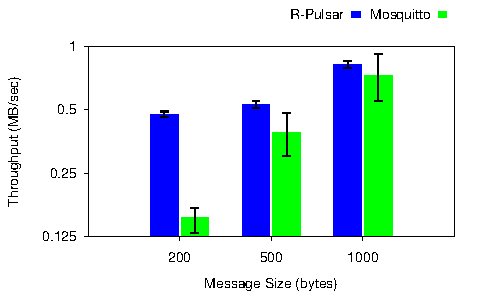
\includegraphics[width=0.8\textwidth]{Results/ProducerPhone}
  \caption{Single broker and producer throughput performance as message sizes grow. Comparison of R-Pulsar and Mosquitto on the Android system.}
  \label{fig:ProducerPhone}

\end{figure}

\subsection{Scalability of Store/Query Operations Over Cloud Systems}

These experiments are aimed to stress the system and evaluated the storage and query scalability of R-Pulsar using multiple workload sizes. The following workloads were used for the tests: Workload 1 (W1) stored/queried one element, Workload 2 (W2) stored/queried 10 different elements, Workload 3 (W3) stored/queried 50 different elements, and Workload 4 (W4) stored/queried 100 different elements. For this test, all RP nodes were part of the same P2P network and the same geographic region to evaluate how R-Pulsar scales as the number of RP increases in each region. 

\begin{figure}[h!]
  \centering
  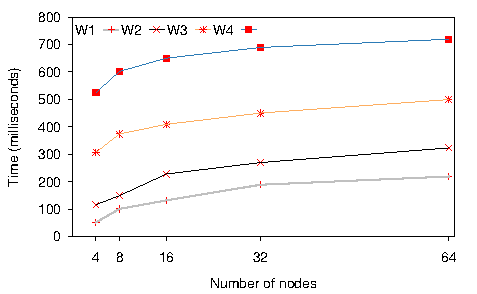
\includegraphics[width=0.8\textwidth]{Results/ProducerLine.pdf}
  \caption{Evaluation of R-Pulsar store query operations as the number of nodes increases on Chameleon cloud.}
  \label{fig:ProducerLine}
\end{figure}

Figure~\ref{fig:ProducerLine} presents the scalability evaluation of the R-Pulsar store operation. The figure shows that for storing a single element (W1), the runtime increased by a factor of $\sim$4 when the system size increased by a factor of 16 (from 4 nodes to 64 nodes). As the system expands, the number of intermediary nodes involved in routing the query grows, causing an increase in the runtime. The storage of 100 different elements (W4) forces the system to store elements in multiple destinations.

\begin{figure}[h!]
  \centering
  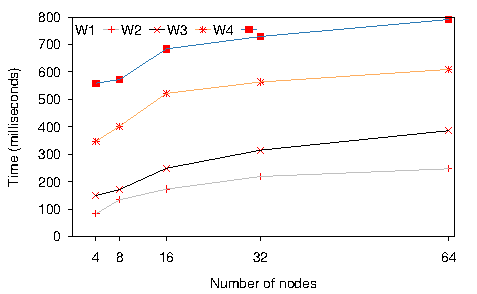
\includegraphics[width=0.8\textwidth]{Results/ProducerLineEx.pdf}
  \caption{Evaluation of R-Pulsar exact query operations as the number of nodes increases on Chameleon Cloud.}
  \label{fig:ProducerLineEx}
\end{figure}

Figure~\ref{fig:ProducerLineEx} presents an evaluation of the exact query operations. It shows that the query of a single element (W1), the runtime increases by a factor of 2.8 when the system size increases by a factor of 16 (from 4 nodes to 64 nodes).

\subsection{Performance of the Query and Store Layer Over Edge Systems}

The next set of experiments explores the performance of the R-Pulsar's storage and query layer as compared to self-contained, embedded and lightweight data storage systems. We compare R-Pulsar with lightweight SQL (SQLite) and non-SQL (NitriteDB) storage systems. We choose SQLite and Nitrite DB because  both systems are designed to be deployed in constrained devices~\cite{sqlite}~\cite{nitrite}. In addition, Nitrite DB is a key-value store like R-Pulsar. 

The experiments were deployed in 10 Raspberry Pis and grouped them together in the same R-Pulsar group. A client then issued requests for data to be stored and queried. As neither Nitrite DB nor SQLite supports horizontal data partitioning, the client directly queried a single DB for these systems. In the case of R-Pulsar, the content-based routing layer is responsible for determining where the data should be stored or queried.

We present three different results for these experiments. Figure~\ref{fig:DBInsertBar} shows the time required for each system to store different sets of elements. R-Pulsar presents a steady performance as the number of elements grows. It also outperforms Nitrite DB (factor of 30x).

\begin{figure}[h!]
  \centering
  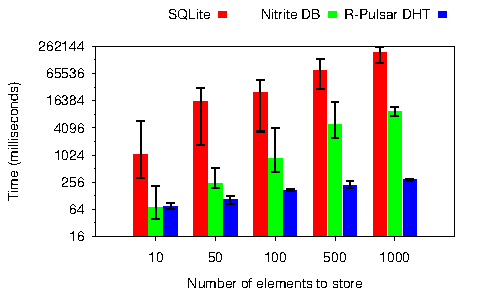
\includegraphics[width=0.8\textwidth]{Results/DBInsertBar}
  \caption{Storage performance of R-Pulsar, SQLite and Nitrite DB as the number of elements to be stored increases over 10 Raspberry Pi.}
  \label{fig:DBInsertBar}
\end{figure}

Figure~\ref{fig:DBExactBar} and~\ref{fig:DBWildBar} present the results for experiments using exact and wildcard queries (a profile containing wildcards, ranges or both).
In the last two experiments, we can observe that Nitrite DB and SQLite are both faster when the number of consecutive reads is small, but R-Pulsar outperforms both when the workload increases. 
Overall, R-Pulsar has a higher performance because it takes advantage of the distributed storage of data over multiple RPs so that queries can be performed in parallel.

\begin{figure}[h!]
  \centering
  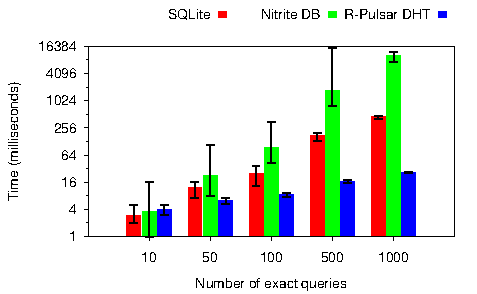
\includegraphics[width=0.8\textwidth]{Results/DBExactBar}
  \caption{Exact query performance of R-Pulsar, SQLite and Nitrite DB as the number of exact queries increases over 10 Raspberry Pi.}
  \label{fig:DBExactBar}
\end{figure}

\begin{figure}[h!]
  \centering
  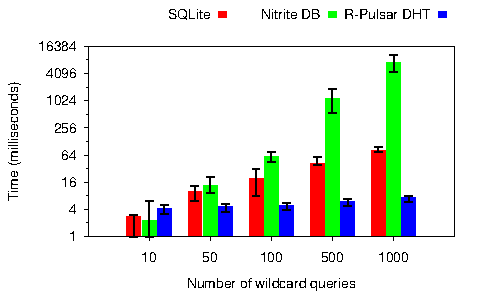
\includegraphics[width=0.8\textwidth]{Results/DBWildBar}
  \caption{Wildcard query performance of R-Pulsar, SQLite and Nitrite DB as the number of wildcard queries increases over 10 Raspberry Pi.}
  \label{fig:DBWildBar}
\end{figure}


\section{Rule-based Programming Abstraction Evaluation}

In this section ....

\subsection{Scalability and Overhead Over Edge and Cloud Systems}

To evaluate the scalability and the overhead of our system we performed two sets of experiments in two types of virtual nodes. The first node is our "drone" with computational capabilities with 1 vCPU and 2 GB of memory, we used a low CPU machine to simulate the overheads as if we used a small IoT device with reduced computational capacity. The second node is the "minivan" with 8 vCPU and 32 GB of memory, we assume that a minivan will be able to carry higher computational resources.

\begin{figure}[h!]
  \centering
  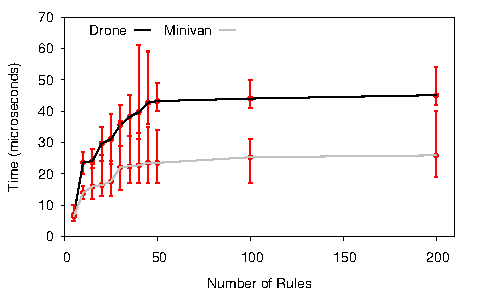
\includegraphics[width=0.8\textwidth]{Results/RuleEngine}
  \caption{Rule engine overhead for different number of rules.}
  \label{fig:RuleEngine}
\end{figure}

To evaluate the scalability and overhead of the rule engine system we added different rule amounts and streamed our regular workload, forcing the evaluation of each of the tuples. The plotted graph in Figure  \ref{fig:RuleEngine} shows the scalability and overhead of our rule engine for two different machines described above. We can observe that the overhead is very minimal and can be used for processing real-time stream processing, we can also observe that as we add rules the overheads do not increase exponentially making it suitable to handle hundreds of rules.

\begin{figure}[h!]
  \centering
  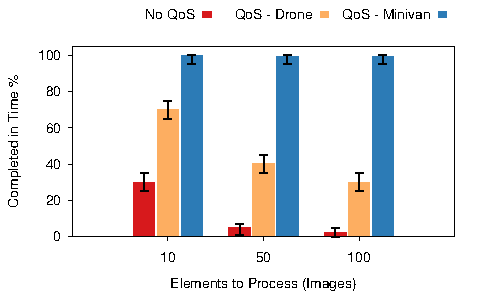
\includegraphics[width=0.8\textwidth]{Results/QoS}
  \caption{Data quality rule-based system 20 second deadline.}
  \label{fig:QoS}
\end{figure}

In this experiment we wanted to show the importance of being able to programmatically express a trade-off between data quality and computational performance. Figure \ref{fig:QoS} we demonstrate that if we do not allow the to specify QoS rules to set a deadline in this case a deadline of 20 seconds per tuple was specified, depending on the workload and the underlying computing capabilities most of the tuples will not satisfy the deadline. We can also see that our algorithm can't guarantee 100\% completion in time in small computational resources, but that is due to the fact that the CPU can't drain the storm bolt queues fast enough, so some tuples will experience some extra delay.

\section{End To End Evaluation}
In this section we implement two of the five uses cases using R-Pulsar to showcase the ability to express and decide what, where and when data gets collected and processed, using edge and cloud resources, and we compared it against a traditional approach of moving all the data to the cloud for analysis.

\subsection{Disaster Response Use Case}

For the disaster response use case we performed a set of experiments to compare the proposed split architecture (edge and core processing) with the current state of the art approach in which the stream processing is located in a fixed location at the core of the infrastructure. To perform these experiments we deployed them all in the same Chameleon cluster and we introduced artificial latency between the edge of the network and the core of the network. For the edge setup, 3 instances of type m1.small simulate computation capabilities of a drone (1 VCPUs and 2 GB of memory) and 3 other instances of type m1.medium simulate the minivan (2 VCPUs and 8 GB of memory). The core of the network is represented by 3 instances of type m1.large (4 CPUs and 8 GB of memory). To simulate that the edge infrastructure was located in a minivan or a drone we stored all the images that need to be processed locally to simulate a small latency since the minivan or the drone will be producing the data. For the traditional approach the storm topology gets the data from an external server to simulate the latencies need it to transfer between the edge and the core of the network.

\begin{figure}[h]
  \centering
  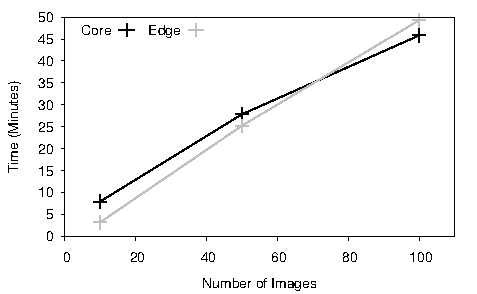
\includegraphics[width=0.8\textwidth]{Results/EdgeVCore}
  \caption{Disaster response workflow edge vs core no QoS.}
  \label{fig:Edge_CoreVsCloud}
\end{figure}

For the experiment in Figure \ref{fig:Edge_CoreVsCloud} we wanted to demonstrate that if we simply deployed our entire workflow at the edge of the network without any "quality" trade-off and we compared it to the traditional approach where each of the LiDAR images will be sent to the core for processing. We can see that with small workflows the edge is significantly faster than the core of the network, but as the number of images that need to be processed grows (the affected area is large) the core performs better than the edge due to limited resources at the edge of the network.

\begin{figure}[h]
  \centering
  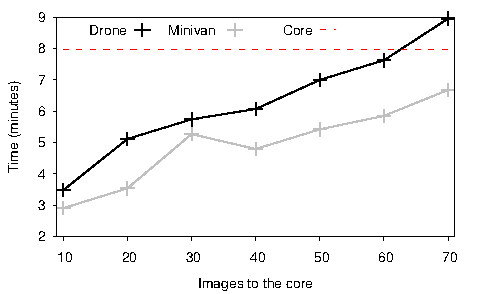
\includegraphics[width=0.8\textwidth]{Results/SmallSpeed}
  \caption{Disaster response workflow 10 images edge speed-up.}
  \label{fig:SmallSpeed}
\end{figure}

\begin{figure}[h]
  \centering
  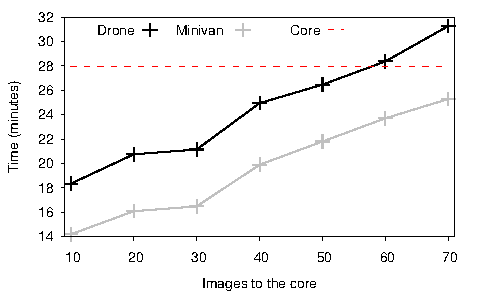
\includegraphics[width=0.8\textwidth]{Results/MediumSpeed}
  \caption{Disaster response workflow 50 images edge speed-up.}
  \label{fig:MediumSpeed}
\end{figure}

\begin{figure}[h]
  \centering
  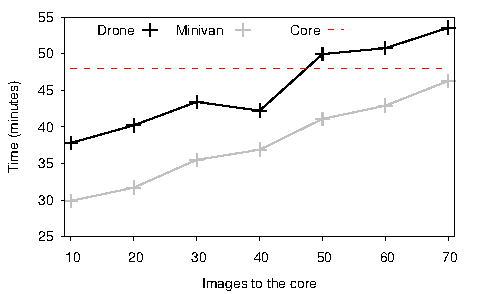
\includegraphics[width=0.8\textwidth]{Results/BigSpeed}
  \caption{Disaster response workflow 100 images edge speed-up.}
  \label{fig:BigSpeed}
\end{figure}

Figures \ref{fig:SmallSpeed} \ref{fig:MediumSpeed} \ref{fig:BigSpeed} showcase the speed-up that can be obtained by trading off some image "quality" for some computational complexity. Figure \ref{fig:SmallSpeed} is the graph for a workflow with 10 LiDAR images to be processed; one can observe that if we perform all the computations in the "drone" and only 10\% of those images need further processing we get a speed up of 44\% compared to sending all 10 images to the core of the network. We can observe from figures \ref{fig:MediumSpeed} \ref{fig:BigSpeed} that due to the small compute limitations, the drone gets a faster speed-up when the worflow size is small and a small percentage of tuples needs further processing, which makes it perfect for assessing affected areas where minivans can't get to due to road blocks. In the case of the minivan, it gets a higher speed-up in all three cases since it has higher computational resources and we can also observe that we can still send a large percentage of rules to the core and we still get a higher speed-up. In the best case the minivan is 71\% faster than the traditional approach where all the images are sent to the cloud.

\subsection{Smart City Use Case}

For the smart city use case we performed a set of experiments to compare the proposed edge stream processing approach with a traditional approach in which the stream processing is located in a fixed location at the core of the infrastructure. To perform these experiments we deployed two streaming frameworks (based on Apache Kafka plus Apache Storm), one in our local cluster and another one in Amazon AWS. In both cases, Apache Kafka and Storm were deployed in a single machine to avoid any additional latency due to communication across machines of a Kafka or Storm cluster. In Amazon AWS, we used an instance of type  t2.2xlarge, which has similar characteristics to the machines in our local cluster (8 CPUs and 32 GB of memory). Note that we do not assume that the edge will be equipped with similar characteristics, we are only using this type of instance for computational comparison only. When using our approach, our framework was deployed across both infrastructures -- i.e. we had two RP nodes exposing the capabilities of each stream engine. We emulated a scenario inspired by the one described in Chapter~\ref{chap:applications} in which a client performs a request to obtain navigation indications. The data-processing workflow (i.e. topology) was composed by three sequential steps (i.e. bolts in Apache Storm terms) that performed some basic data transformations that did not require significant computational time. In our experiments we evaluated the performance of both approaches using three different anonymized workloads consisting of 100, 1000, and 10000 data elements. Each data element is around 1KB of size and is generated sequentially. The client and data source were close to our local cluster. Figures~\ref{fig:perf2} and~\ref{fig:perf1} collect the results of these experiments.

\begin{figure}[h]
  \centering
    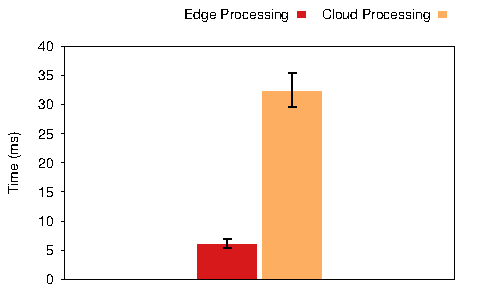
\includegraphics[width=0.8\textwidth]{Figures/Latency.pdf}
  \caption{Delay in processing a data element.} \label{fig:perf2}
\end{figure}
\begin{figure}[h]
  \centering
  	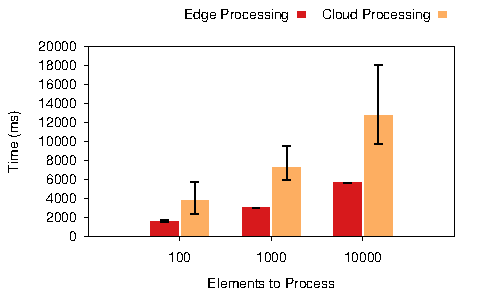
\includegraphics[width=0.8\textwidth]{Figures/EdgeVsCloud.pdf}
  \caption{Completion time for different workloads.} \label{fig:perf1}
\end{figure}

Figure~\ref{fig:perf2} shows the delay in processing a data element. The delay is measured as the time spent between the data producer generates the data element and the destination queue receives it for processing. We observe that in our case, the latency is up to 78\% less than a traditional approach consisting of sending data for processing to a cloud. The main reason is that our approach is able to dynamically identify different sources of computation and data using the location of the client. Therefore, it chooses to process the data in the place that is closest to the data source and the client. Our approach still incurs some small overheads as we have to identify the best processing site and data has to travel from source to destination. Nonetheless, these overheads are negligible compared with those incurred when transferring data between the edge and the core of the infrastructure.

Figure~\ref{fig:perf1} collects the computational time required to process a stream of data elements. We can observe that our approach is up to 56\% more efficient than a traditional cloud-based approach. In this particular case, this is directly related to the delay mentioned before that the system incurs when processing each data element. Since the delay of each data element is larger than its computational time, the system is often idle waiting for small periods of time until a new data element arrives.